\documentclass[xcolor=table, 10pt, aspectratio=169]{beamer}

%\usepackage{arev}
\usepackage{amsmath,amssymb,amscd}
\usepackage{dsfont}
\usepackage{mathrsfs}
\usepackage{yfonts}
\usepackage{bm}
\usepackage{graphicx}
\usepackage{tabularx}
\usepackage{animate}
%\usepackage{ifthen}

%\usepackage{xeCJK}
%\usepackage{fontspec}
%\newfontfamily\cjkfont{PingFang SC}
%\setCJKmainfont{PingFang SC}
\newcolumntype{x}{>{\centering\arraybackslash}X}
\renewcommand{\arraystretch}{1.5}

\usepackage{tikz}
	\usetikzlibrary{calc}
	\usetikzlibrary{arrows,shapes, positioning, matrix}
	\usetikzlibrary{decorations.markings}
	\tikzstyle arrowstyle=[scale=1]
	\tikzstyle directed=[postaction={decorate,decoration={markings,
 	   mark=at position .15 with {\arrow[arrowstyle]{stealth}}}}]
\tikzstyle string=[thick,postaction={decorate,decoration={markings,
    mark=at position .55 with {\arrow[arrowstyle]{stealth}}}}]
\tikzstyle dual_string=[dashed,postaction={decorate,decoration={markings,
    mark=at position .55 with {\arrow[arrowstyle]{stealth}}}}]

\tikzstyle dw=[thick,postaction={decorate,decoration={markings,
    mark=at position 1 with {\arrow[arrowstyle]{stealth}}}}]
\tikzstyle group=[mbg]

\usepackage{pgffor}
\newcommand{\mb}[1]{\mathbf{#1}}
\renewcommand{\cal}[1]{\mathcal{#1}}

\newcommand{\ag}[2]{#1_\mb{#2}}
\newcommand{\cohosub}[1]{\scalebox{0.72}{\textswab{#1}}}
\newcommand{\cohosubsub}[1]{\scalebox{0.6}{\textswab{#1}}}
\newcommand{\coho}[1]{\textswab{#1}}


\mode<presentation>
{
  %\usetheme{Warsaw}
  % or ...
  %\useoutertheme{rectangle}
  \setbeamertemplate{frametitle}[default][center]
  \defbeamertemplate{itemize item}{flat}{\begin{pgfpicture}{-1ex}{0ex}{1ex}{2ex}
      \pgfpathcircle{\pgfpoint{0pt}{.6ex}}{0.6ex}
      \pgfusepath{fill}
    \end{pgfpicture}%
  }
  \defbeamertemplate{itemize subitem}{flat}{\footnotesize\raise0.5pt\hbox{\textbullet}}
  \defbeamertemplate{itemize subsubitem}{flat}{\footnotesize\raise0.5pt\hbox{\textbullet}}

  %\useinnertheme{circles}
  \setbeamertemplate{items}[flat]
  \setbeamertemplate{sections/subsections in toc}[circle]
  \setbeamertemplate{blocks}[rounded]
  \setbeamertemplate{title page}[default][colsep=-4bp,rounded=true]
  \setbeamertemplate{part page}[default][colsep=-4bp,rounded=true]
  \setbeamercovered{transparent}
  %\usecolortheme{spruce}
  %\definecolor{THU}{RGB}{116,61,130}
  \definecolor{mbg}{RGB}{0,0,160}
  \setbeamercolor*{palette primary}{fg=white,bg=mbg}
  \setbeamercolor*{titlelike}{parent=palette primary}
  \setbeamercolor*{structure}{fg=mbg}
  \setbeamercolor{frametitle}{fg=white,bg=mbg}
  % or whatever (possibly just delete it)
  \setbeamercolor{block title}{bg=mbg,fg=white}
  \setbeamercolor{block body}{bg=mbg!15}


  \addtobeamertemplate{navigation symbols}{}{ \hspace{1em}%
    \usebeamerfont{footline}%
    \insertframenumber / \inserttotalframenumber }
}


%\usepackage[english]{babel}
% or whatever

%\usepackage[latin1]{inputenc}
% or whatever

%\usepackage{times}
%\usepackage[T1]{fontenc}
% Or whatever. Note that the encoding and the font should match. If T1
% does not look nice, try deleting the line with the fontenc.

\title[U1SL] % (optional, use only with long paper titles)
{Monte Carlo Study of Compact Quantum QED with Fermionic Matter [2+1D U(1)-Dirac Spin Liquid]}

\author[Y Qi] % (optional, use only with lots of authors)
{Yang~Qi}
% - Give the names in the same order as the appear in the paper.
% - Use the \inst{?} command only if the authors have different
%   affiliation.

\institute[Fudan] % (optional, but mostly needed)
{
Department of Physics, Fudan University.
}
% - Use the \inst command only if there are several affiliations.
% - Keep it simple, no one is interested in your street address.

%\date{2016 Annual Meeting of Fudan CFTPP} % (optional, should be abbreviation of conference name)
%{Fudan University, Oct 13 2015}
\date{APS March Meeting, Boston, Mar. 2019.}
% - Either use conference name or its abbreviation.
% - Not really informative to the audience, more for people (including
%   yourself) who are reading the slides online

\subject{Theoretical Physics}
% This is only inserted into the PDF information catalog. Can be left
% out.



% If you have a file called "university-logo-filename.xxx", where xxx
% is a graphic format that can be processed by latex or pdflatex,
% resp., then you can add a logo as follows:

\pgfdeclareimage[height=1cm]{university-logo}{../resources/fudan}
\logo{\pgfuseimage{university-logo}}



% Delete this, if you do not want the table of contents to pop up at
% the beginning of each subsection:
\AtBeginSection[]
{
  \begin{frame}<beamer>{Outline}
			\tableofcontents[currentsection,currentsubsection]
  \end{frame}
}
%\AtBeginSubsection[]
%{
 % \begin{frame}<beamer>{Outline}
  %  \tableofcontents[currentsection,currentsubsection]
  %\end{frame}
%}


\begin{document}

\begin{frame}
  \titlepage
\end{frame}

\begin{frame}{Collaborators}
\begin{itemize}
\item Xiao Yan Xu, Hong Kong University of Science and Technology.
\item Zi Yang Meng, Institute of Physics, Beijing.
\item Long Zhang, Kavli Institute for Theoretical Sciences, UCAS, Beijing.
\item Fakher F. Assaad, Universit\"at W\"urzburg.
\item Cenke Xu, University of California, Santa Barbara.
\begin{center}
  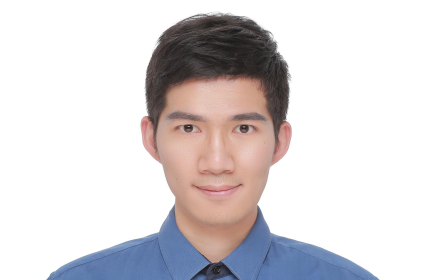
\includegraphics[height=2cm]{../people/xiaoyanxu}
  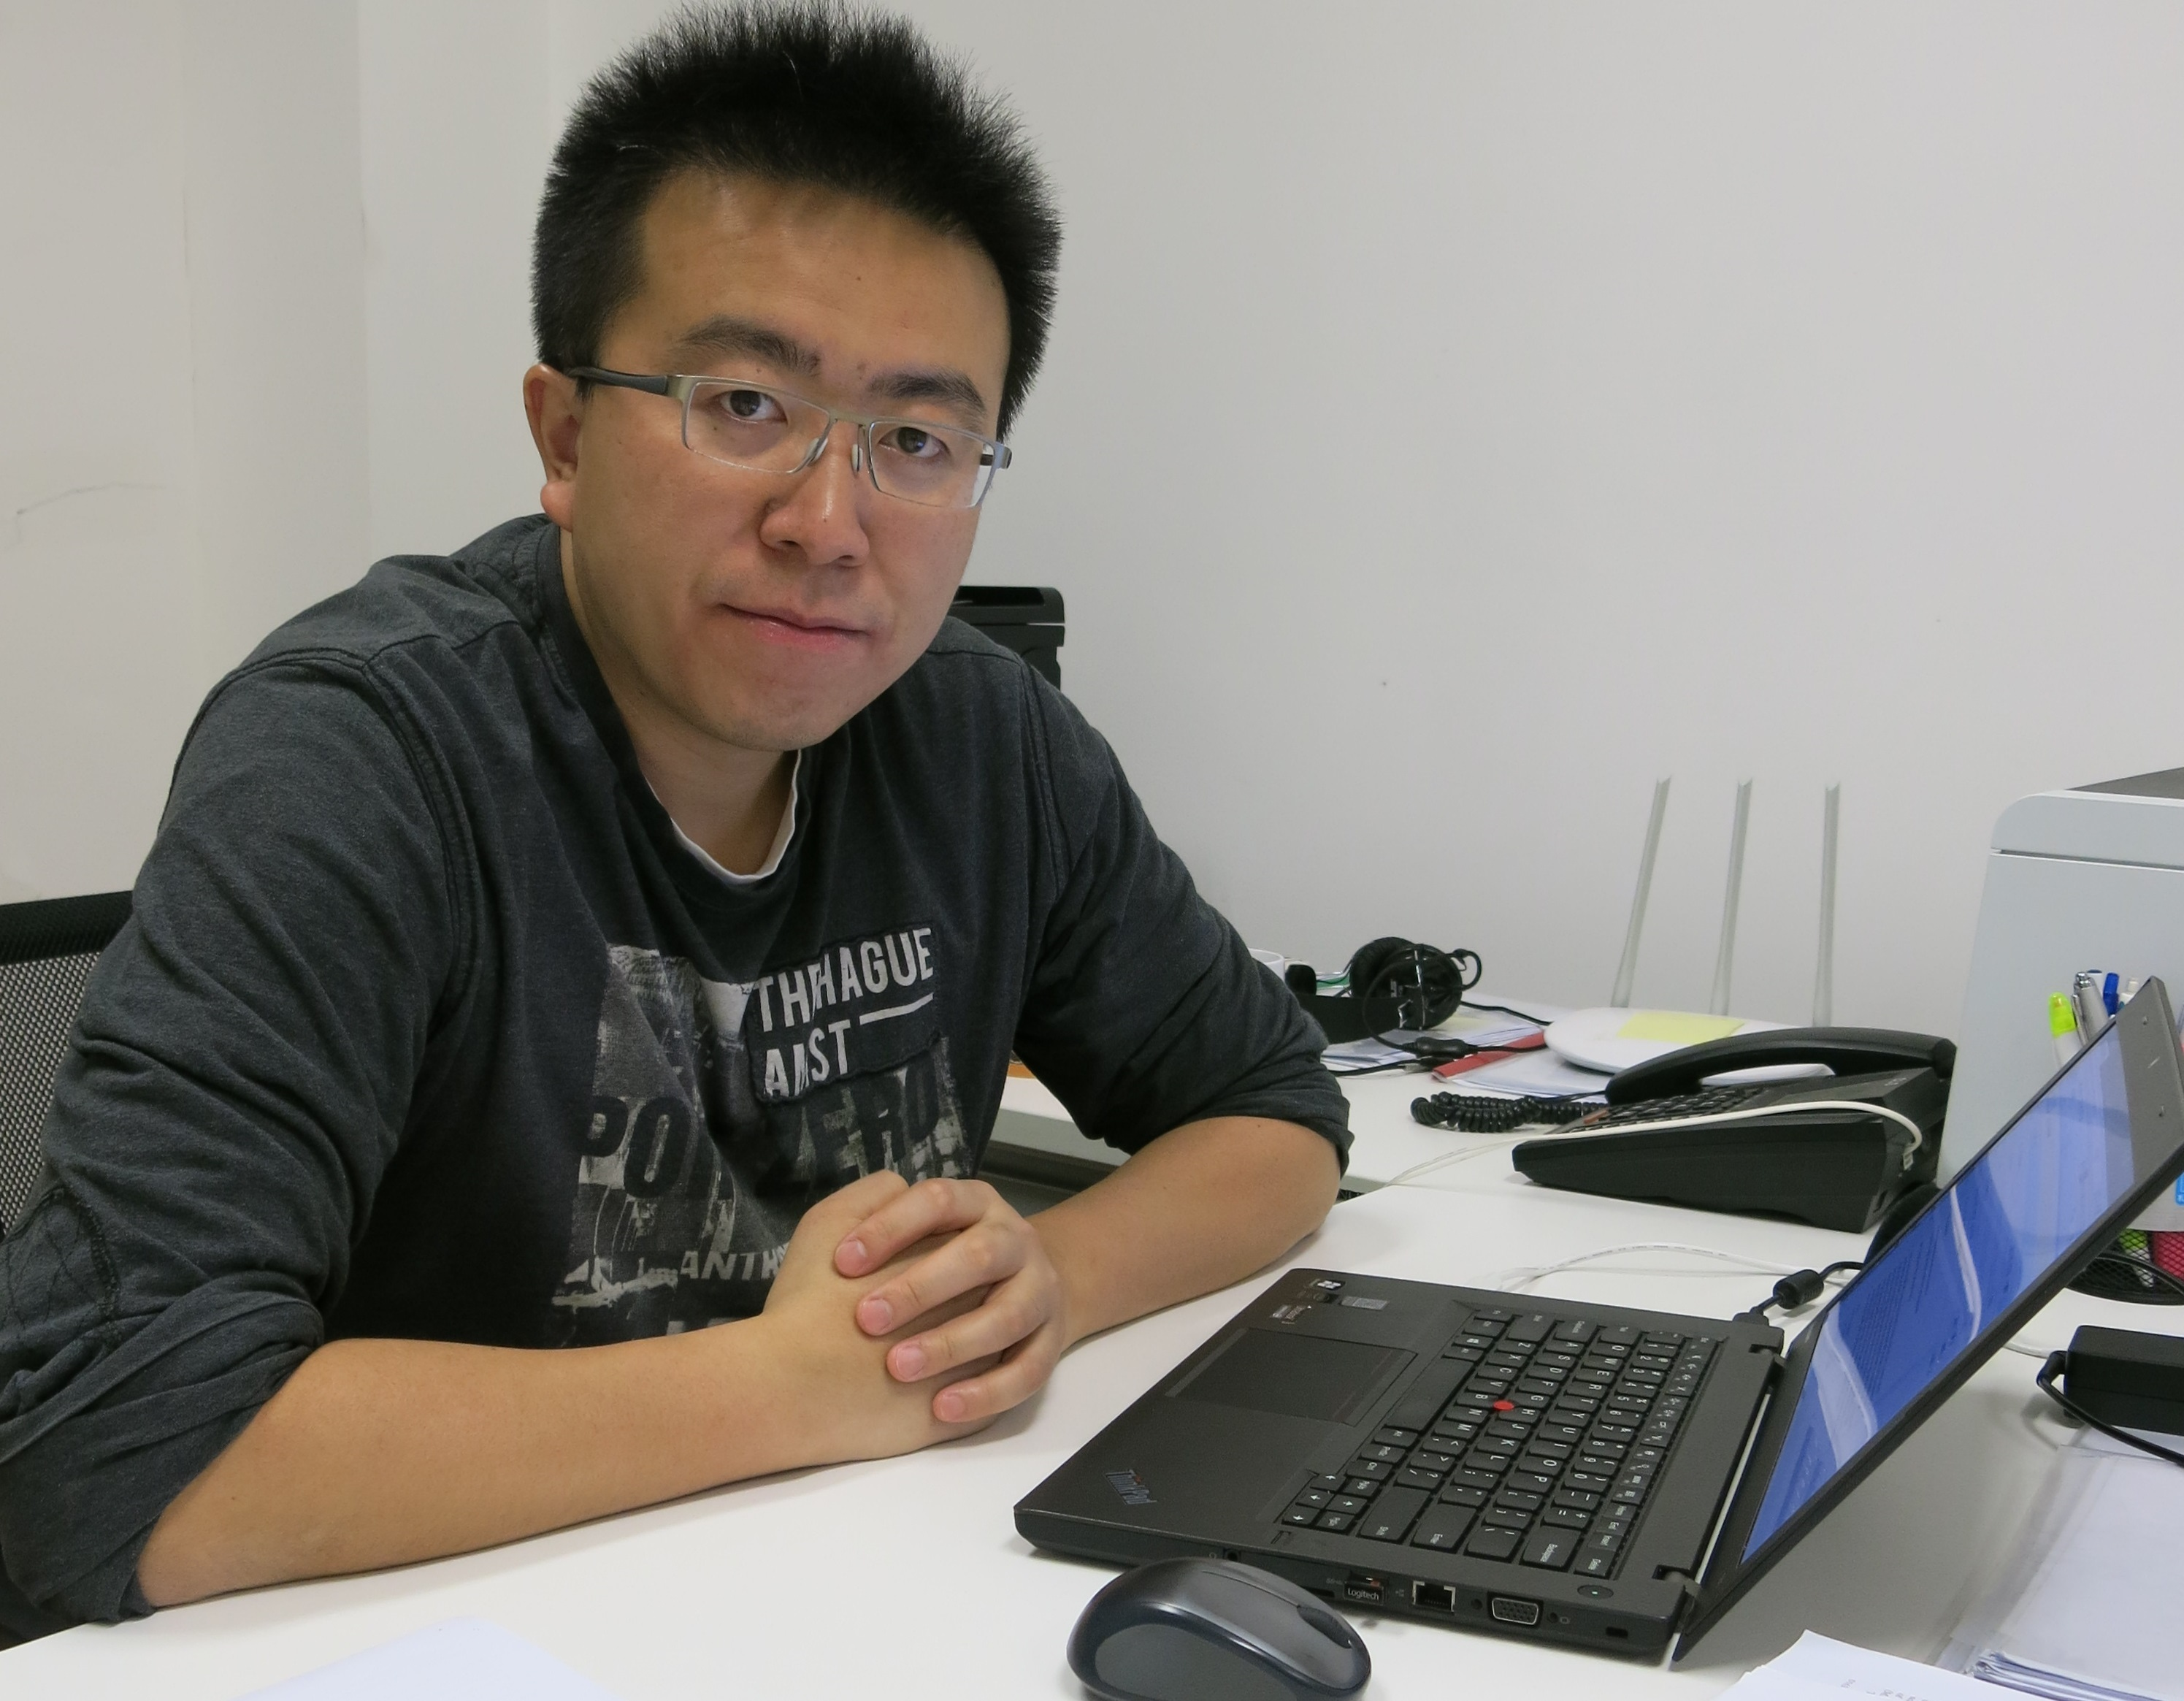
\includegraphics[height=2cm]{../people/ziyangmeng}\\
  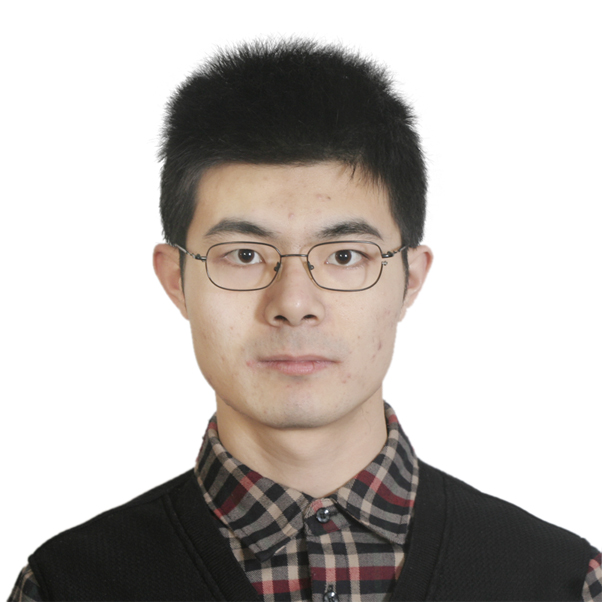
\includegraphics[height=2cm]{../people/zhanglong}
  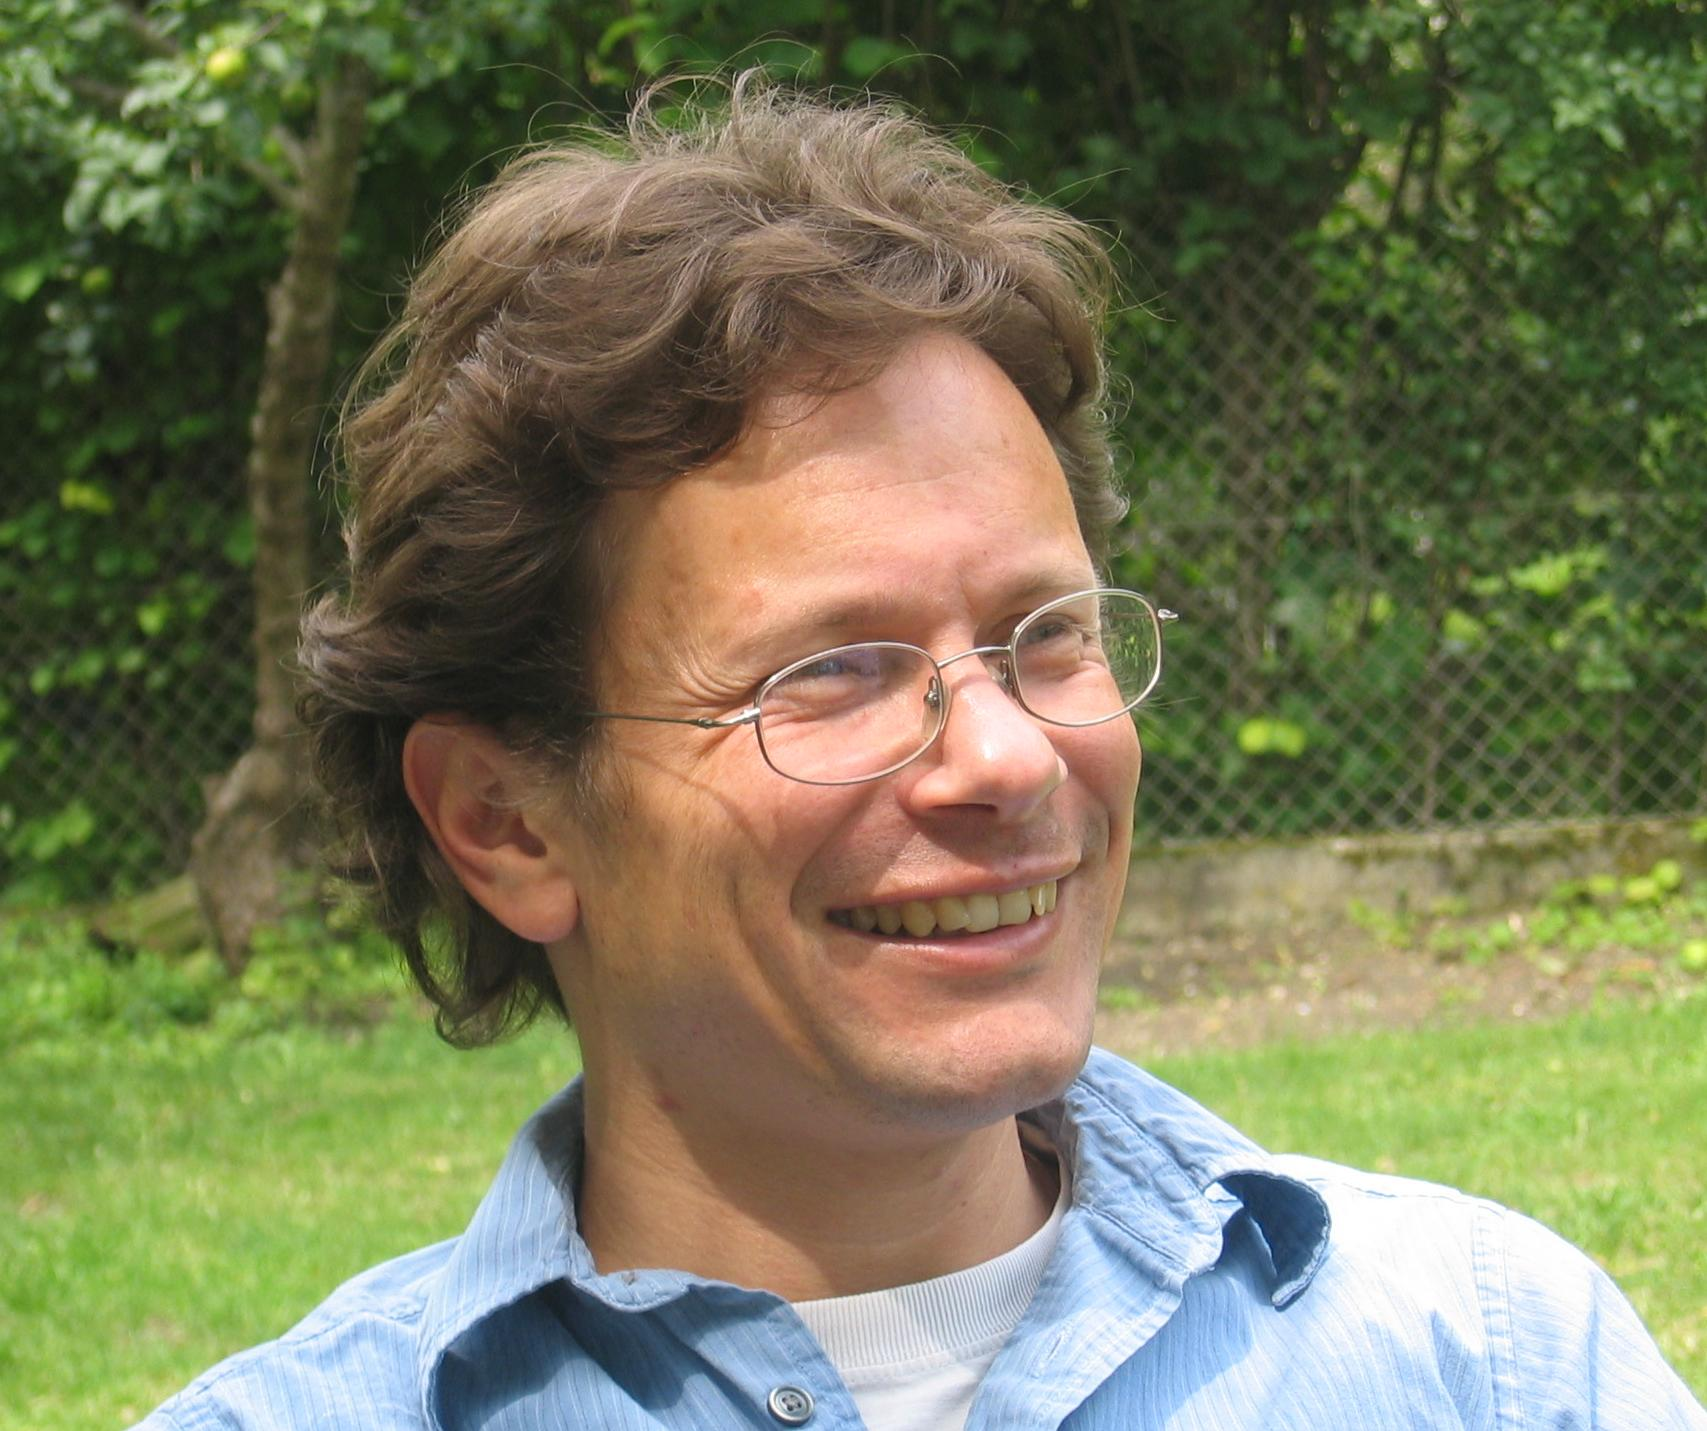
\includegraphics[height=2cm]{../people/fakher}
  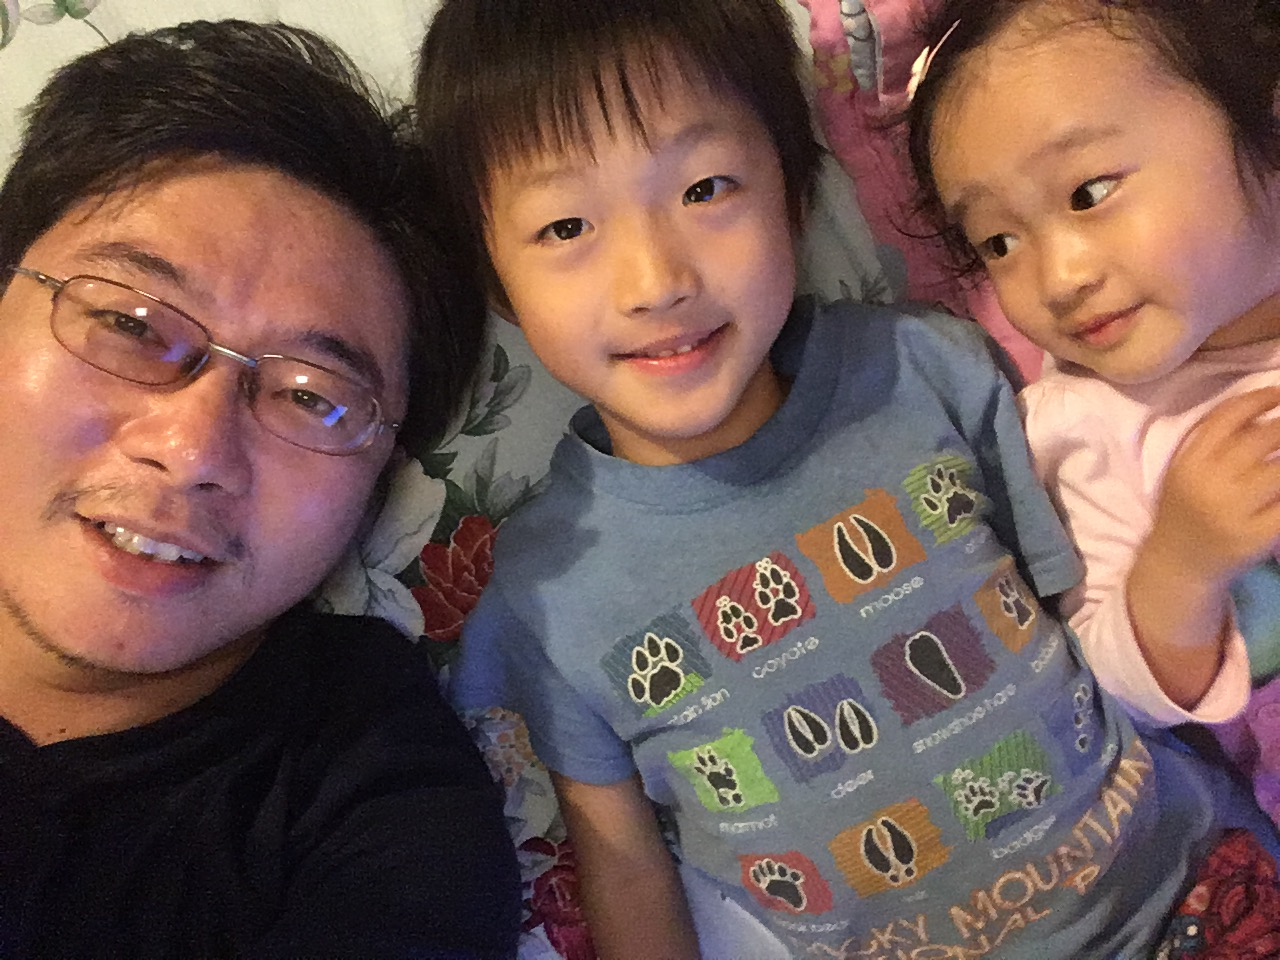
\includegraphics[height=2cm]{../people/cenke}
\end{center}
\end{itemize}
\begin{center}
  \small Phys. Rev. X \textbf{9}, 021022 (2019).
\end{center}
\end{frame}

\begin{frame}{Outline}
	%\begin{columns}
	%\column{.7\textwidth}
		\tableofcontents
  %\end{columns}
  % You might wish to add the option [pausesections]
\end{frame}

\section{Introduction}

\begin{frame}
  \frametitle{U(1) Quantum Spin Liquid: History and Outlooks}
\begin{itemize}
	\item U(1)-Dirac spin liquid: Dirac-fermion spinons + U(1) gauge field.
	\[\mathcal L = \bar\psi_\alpha \gamma^\mu(\partial_\mu-iA_\mu)\psi +  F_{\mu\nu}^2,\quad
	\vec S_i = \psi^\dagger_{i\alpha}\vec\sigma_{\alpha\beta}\psi_{i\beta}.\]
	\item $\pi$-flux phase in high-$T_c$ cuprates:\\
	\emph{\small I. Affleck and J. B. Marston, Phys. Rev. B 37, 3774 (1988).}
	\item Spin liquid in frustrated magnets: kagome-lattice Heisenberg model?\\
	\emph{\small Y. Ran, M. Hermele, P. A. Lee, and X.-G. Wen, Phys. Rev. Lett. 98, 117205 (2007).}

  \item Does the mean-field picture stand: Is the U(1) gauge field deconfined?
\end{itemize}
\end{frame}

%\begin{frame}
%  \frametitle{Compact U(1): Monopoles}
%  \begin{itemize}
%    \item Gauge theory in the continuum:
%    \[S=\int d^3x (\epsilon_{abc}A_c)^2.\]
%    \item Gauge theory on a lattice:
%    \[S=\sum_{\square}e^{iA_{ij}}e^{iA_{jk}}e^{iA_{kl}}e^{iA_{li}}.\]
%    \item Compact U(1) gauge connection: $A_{ij}\simeq A_{ij}+2\pi$.
%    \item Monopole: non-smooth space-time configurations of $A_{ij}$.
%    \item Even without matter field, compact U(1) is not free Maxwell theory: confinement in the IR.
%  \end{itemize}
%\end{frame}

\begin{frame}
	\frametitle{Does U(1) spin liquid exist in 2+1D?}
	\[\mathcal L = \bar\psi_\alpha \gamma^\mu(\partial_\mu-iA_\mu)\psi + F_{\mu\nu}^2.\]
	\begin{itemize}
		\item U(1) monopole: confinement. Compact U(1) is \alert{not free}.
		\item Gapless fermions suppress monopole.
	\end{itemize}
	\begin{tabular}{p{.3\textwidth}p{.3\textwidth}p{.3\textwidth}}
		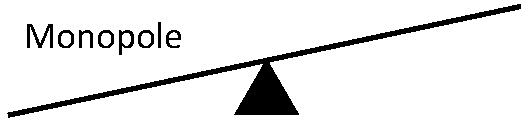
\includegraphics[scale=.45]{balance1}
		&
		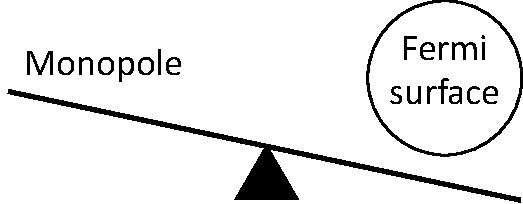
\includegraphics[scale=.45]{balance2}
		&
		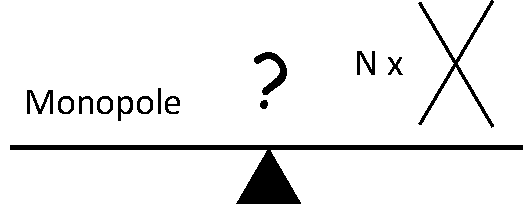
\includegraphics[scale=.45]{balance3}\\
		Pure compact U(1). & Spinon FS. & A critical $N_f$?\\
		A. M. Polyakov, Gauge fields and strings. & Sung-Sik Lee, PRB 78 085129 (2008). & Under heavy debate: large-$N_f$ expansion / CFT argument / numerical simulations.
	\end{tabular}
\end{frame}

\begin{frame}
	\frametitle{Our Approach}
	\[H = \sum_{ij}\vec S_i\cdot\vec S_j+\cdots
	\quad\Rightarrow\quad
	\mathcal L = \bar\psi_\alpha \gamma^\mu(\partial_\mu-iA_\mu)\psi
	+ F_{\mu\nu}^2.
	\quad\Rightarrow\quad\text{Confinement??}\]
	\begin{itemize}
		\item Use a model Hamiltonian to study the QED$_3$ theory in the IR.
		\item Not worrying which realistic spin Hamiltonian can realize it.
		\item Similar to previous studies on $\mathbb Z_2$ Dirac spin liquids:
		\emph{F. F. Assaad and Tarun Grover, PRX 2016; Snir Gazit, Mohit Randeria, and Ashvin Vishwanath, Nat Phys 2017.}
	\end{itemize}
\end{frame}

\section{Model and Method}

\begin{frame}
  \frametitle{The Model Hamiltonian}
  \[
  H=\frac{1}{2}JN_{f}\sum_{\langle i,j \rangle} \frac 1 4 \hat{L}^{2}_{ij}-t\sum_{\langle i,j \rangle\alpha}\left(\hat{c}^{\dagger}_{i\alpha}e^{i\hat{\theta}_{ij}}\hat{c}_{j\alpha}+\text{h.c.}\right)
  +\ \frac{1}{2}K\ N_f\sum_{\square}\cos \left( \text{curl} \hat{\theta} \right).
\]
\begin{columns}
  \column{.8\textwidth}
  \begin{itemize}
    \item $c$: spinon.
    \item $\theta_{ij}$: quantum rotors $\Rightarrow$ compact gauge field.
    \item $[L_{ij}, e^{i\theta_{ij}}]=e^{i\theta_{ij}}$ is the angular momentum / electric field.
    \item Gauge symmetry:
    \[\hat{Q}_{i} = -\sum_{j}\hat{L}_{ij} + \sum_{\alpha} \left( \hat{c}^{\dagger}_{i\alpha}\hat{c}^{\phantom\dagger}_{i\alpha} - 1/2 \right);[H, \hat Q_i] = 0.\]
    \item Dynamically generated constraint:
		$\hat Q_i \simeq 0$ implies gauge symmetry.
    \item $K>0$ favors a $\pi$-flux state.
		\item $N_f=1$: two Dirac cones (two valley). $N_f=2,4,6,\ldots$ do not have sign problem.
  \end{itemize}

  \column{.2\textwidth}
  \begin{center}
    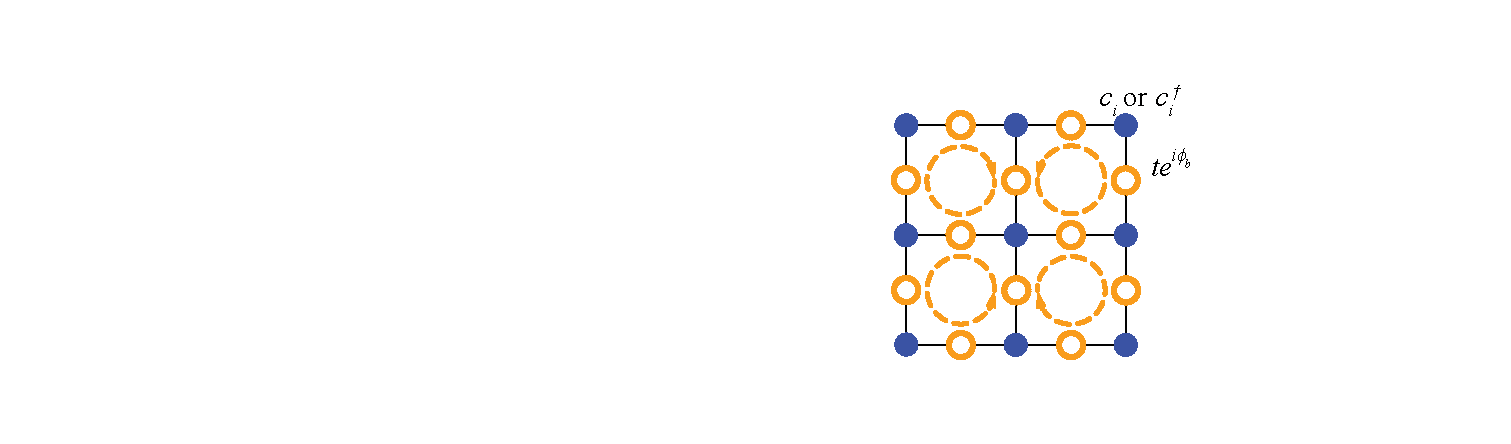
\includegraphics[width=3cm]{model}
  \end{center}
\end{columns}
\end{frame}

%\begin{frame}
%  \frametitle{Dynamically generated constraint}
%  \[C_{Q} = \frac{1}{L^2} \sum_{ij} \langle \hat{Q}_i \hat{Q}_j\rangle,\quad C_Q\rightarrow0\text{ as }\beta\propto L\rightarrow0\].
%  \begin{center}
%    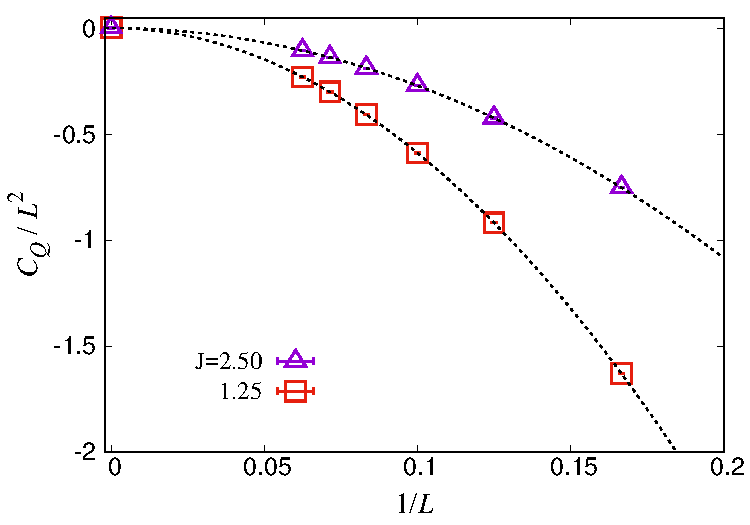
\includegraphics[width=.5\textwidth]{n2QQ00}
%
%		$Q\rightarrow 0$: emergent gauge symmetry.
%  \end{center}
%\end{frame}

\begin{frame}
  \frametitle{The Determinant Quantum Monte Carlo Method}
  \begin{align*}
  L_F &= \sum_{\langle i,j \rangle\alpha}{\psi}^{\dagger}_{i\alpha} \left[(\partial_\tau -\mu)\delta_{ij}-t e^{i\phi_{ij}}   \right]   {\psi}_{j\alpha} + \text{h.c.}\\
  L_\phi &= \frac{4} {JN_{f}\Delta \tau ^2} \sum_{\langle i,j \rangle}
  \left[ 1-\cos(\phi_{ij}(\tau+1)-\phi_{ij}(\tau))
   +\frac{1}{2}K N_f\sum_{\square}\cos (\text{curl} \phi) \right],
\end{align*}
\begin{itemize}
  \item Sampling bosonic configuration: $\phi = \{\phi_{ij}(\tau)\}$.
  \item Weight:
  \[W[\phi] = W_b[\phi]\det(\mathbf I + \mathbf B(\beta,0;\phi))\]
  \item Complexity: $O(\beta N^3)$.
  \item Metropolis Algorithm and Fast Update:
  \[\phi_{ij}(\tau)\rightarrow\phi_{ij}(\tau)+\delta\phi;\quad p(\delta\phi)\propto e^{-\delta\phi^2/(2\Delta^2)}\].
\end{itemize}
\end{frame}

\section{Results}

\begin{frame}
  \frametitle{Phase diagrams}
  \begin{center}
    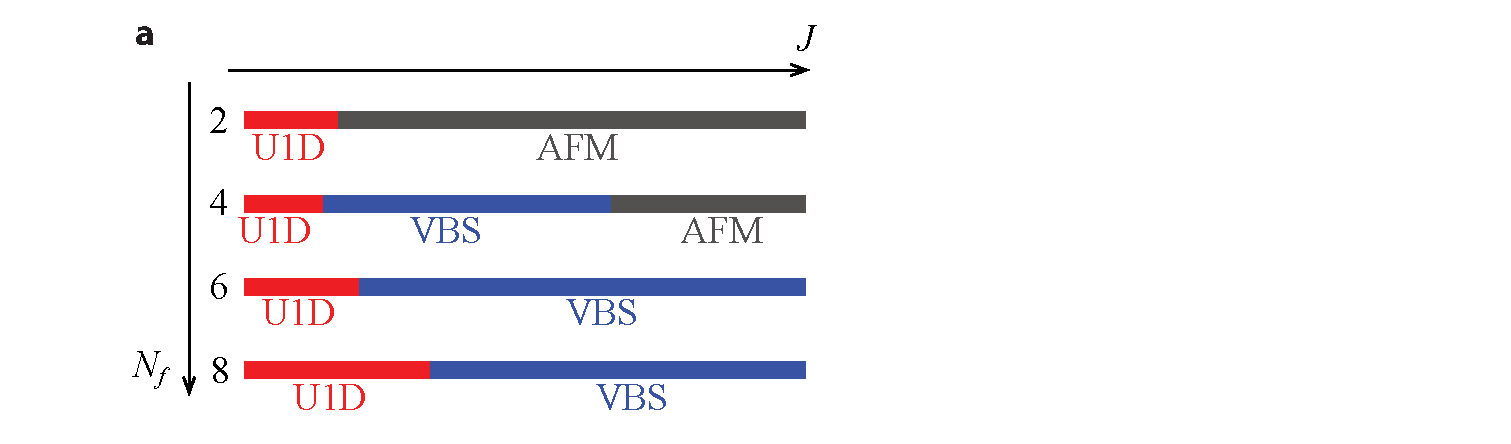
\includegraphics[width=5cm]{phase-diagram}
  \end{center}
  \begin{columns}[t]
    \column{.5\textwidth}
    \begin{block}{U(1)-Dirac Spin Liquid}
      \begin{itemize}
        \item Deconfined U(1) gauge field.
        \item Power-law spin-spin and dimer-dimer correlation functions.
        \item Algebraic spin liquid.
      \end{itemize}
    \end{block}

    \column{.5\textwidth}
    \begin{block}{Confinement phases}
      \begin{itemize}
        \item VBS or AFM long-range order.
        \item Fermion gapped.
        \item Confined U(1) gauge field.
      \end{itemize}
    \end{block}
  \end{columns}
\end{frame}

\begin{frame}
  \frametitle{$N_f=2$: phase boundary}
  \begin{columns}
		\column{.7\textwidth}
    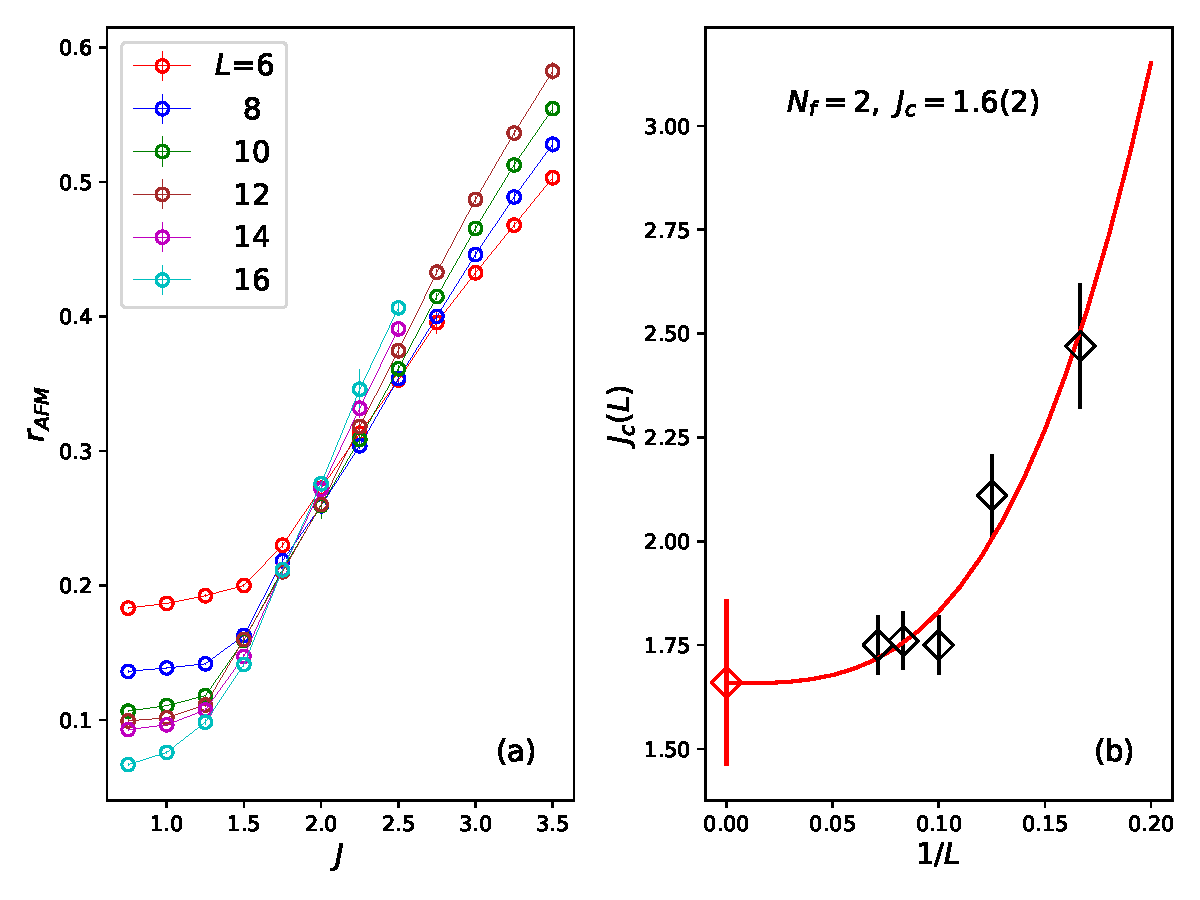
\includegraphics[width=\textwidth]{n2rafm}
		\column{.3\textwidth}
		\begin{itemize}
			\item Correlation ratio: $r = 1-\frac{\chi(\bm Q+\delta\bm q)}{\chi(\bm Q)}.$
			\item Crossing indicates the position of phase transition.
			\item Phase transition b/w U1D and AFM: $J_c=1.6(2)$.
		\end{itemize}
  \end{columns}
\end{frame}

\begin{frame}
  \frametitle{Deconfined U(1) gauge field}
  \begin{columns}
		\column{.6\textwidth}
    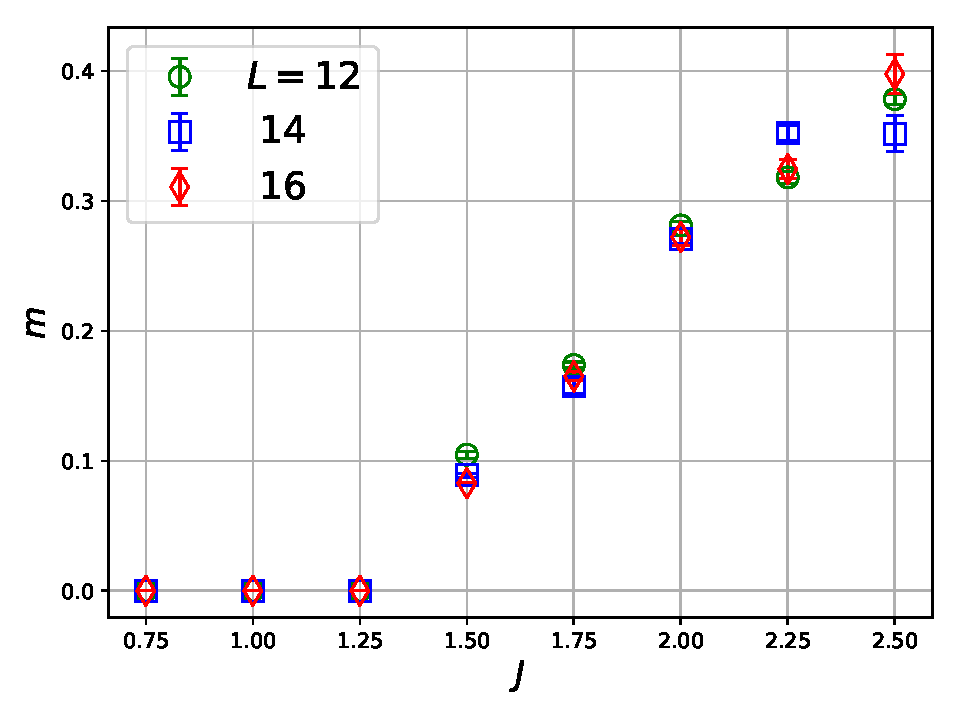
\includegraphics[width=\textwidth]{photonmass}
		\column{.4\textwidth}
		\begin{itemize}
			\item Measure photon mass $m$ from decaying of gauge-flux correlation functions.
			\item $m > 0$: confinement phase.
		\end{itemize}
  \end{columns}
\end{frame}

\begin{frame}
  \frametitle{$N_f=2$: U1D phase}
  \begin{columns}
		\column{.5\textwidth}
    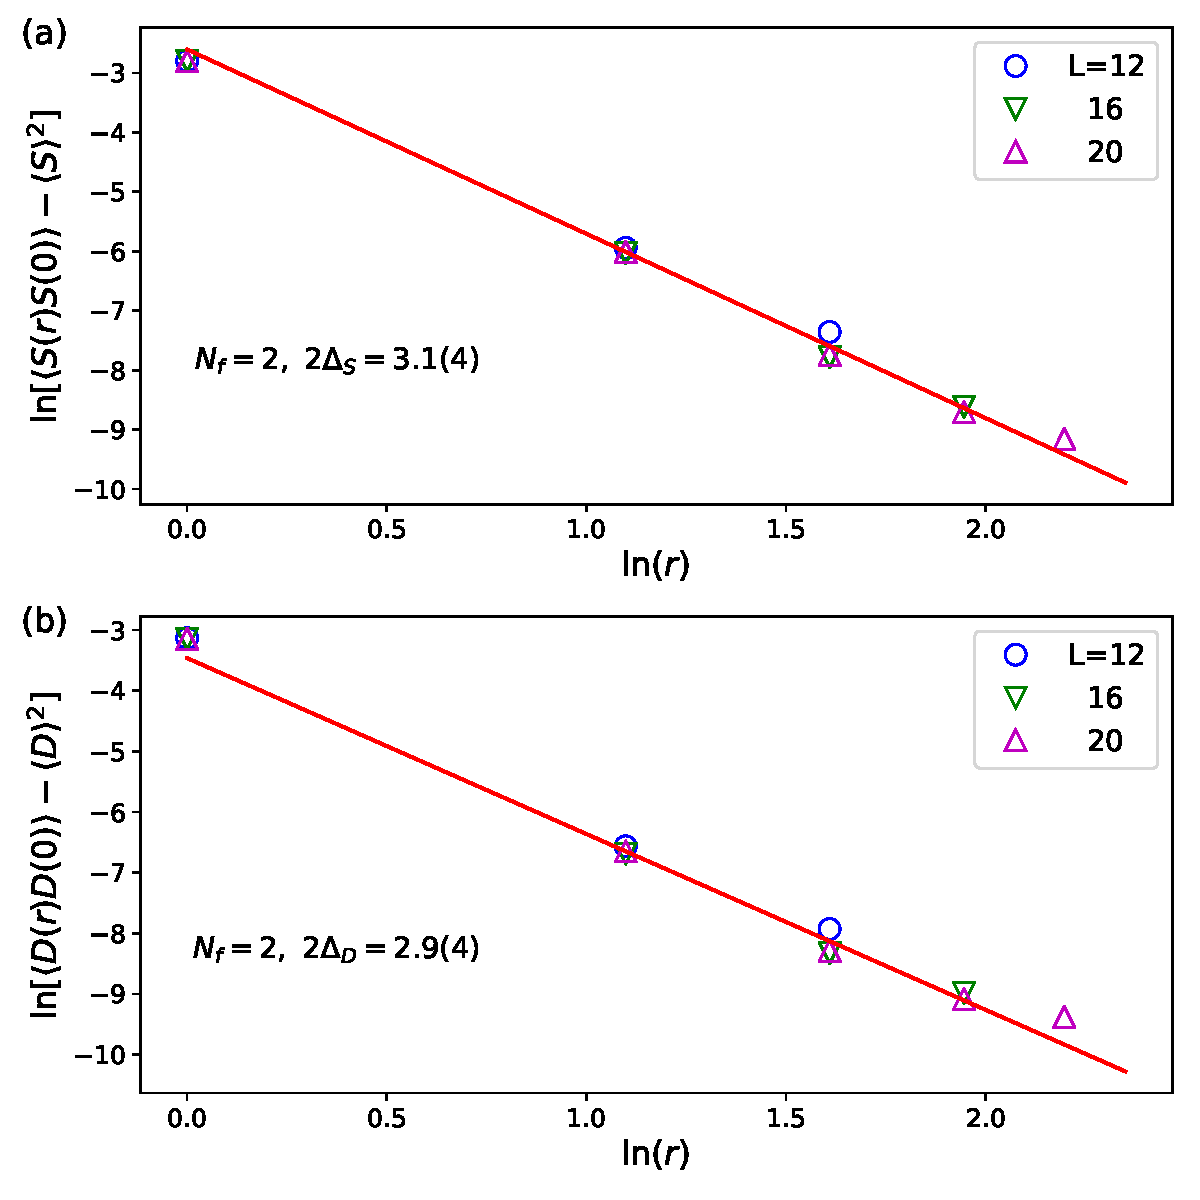
\includegraphics[width=\textwidth]{n2decay}
		\column{.5\textwidth}
		\begin{itemize}
			\item Spin and dimer OPs are fermion bilinears:
			\[\vec S = \psi^\dagger_{i\alpha}\vec\sigma_{\alpha\beta}\psi_{i\beta},\]
			\[D_{x,y} = \psi^\dagger_{i\alpha}\psi_{i+x,y,\beta}.\]
			\item Algebraic spin liquid: $\Delta_S = \Delta_D$.
		  \item (Free fermion has $\Delta_S=\Delta_D = 4$.)
		\end{itemize}
  \end{columns}
\end{frame}

\begin{frame}
  \frametitle{$N_f=4$: phase boundary}
  \begin{columns}
		\column{.7\textwidth}
    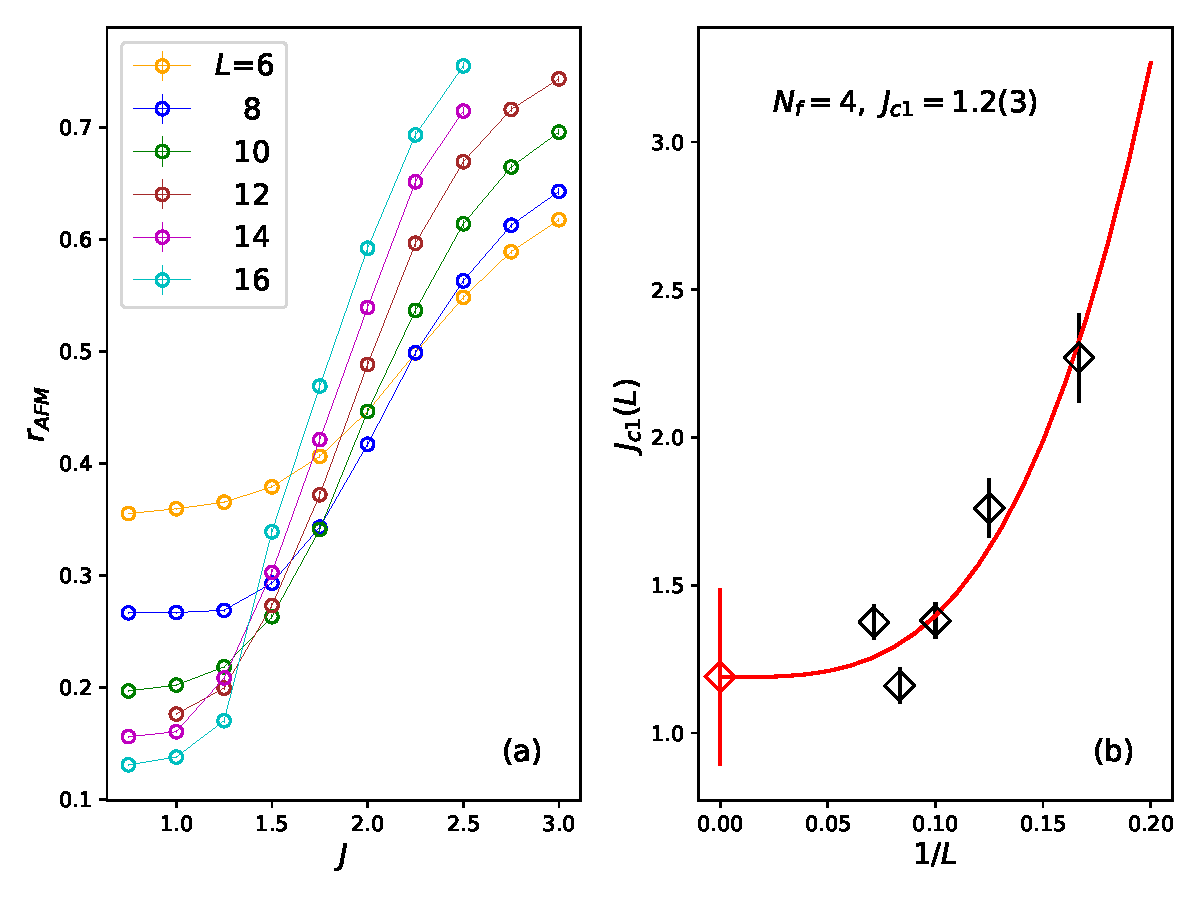
\includegraphics[width=\textwidth]{n4rvbs}
		\column{.3\textwidth}
		\begin{itemize}
			\item Phase transition b/w U1D and VBS: $J_c=1.2(3)$.
		\end{itemize}
  \end{columns}
\end{frame}

\begin{frame}
  \frametitle{$N_f=4$: U1D phase}
  \begin{columns}
		\column{.5\textwidth}
    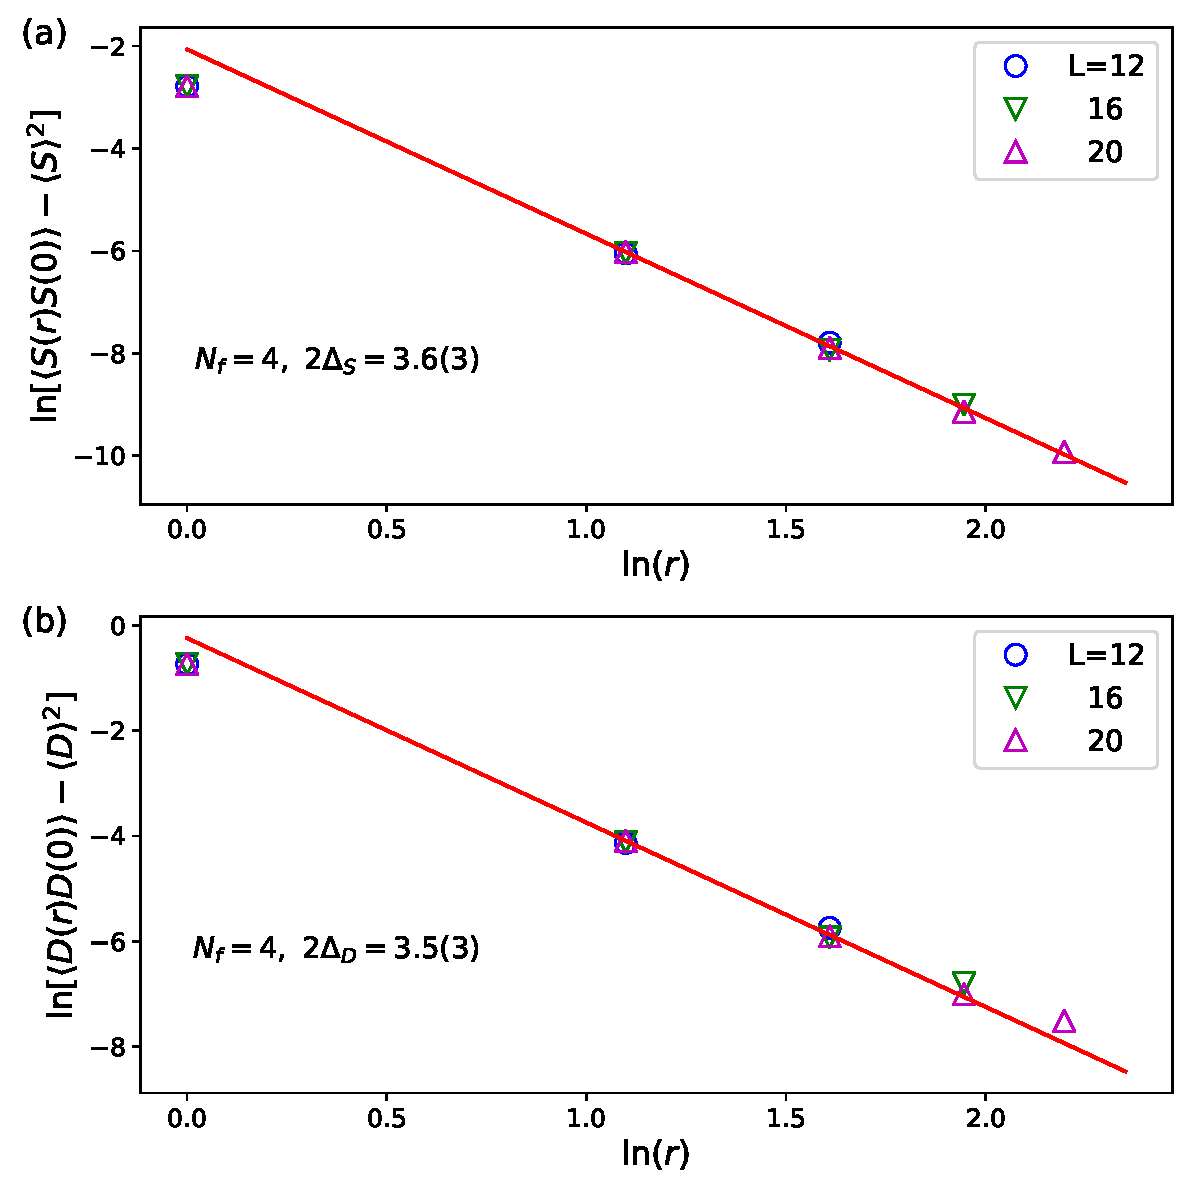
\includegraphics[width=\textwidth]{n4decay}
		\column{.5\textwidth}
		\begin{itemize}
			\item Spin and dimer OPs are fermion bilinears:
			\[\vec S = \psi^\dagger_{i\alpha}\vec\sigma_{\alpha\beta}\psi_{i\beta},\]
			\[D_{x,y} = \psi^\dagger_{i\alpha}\psi_{i+x,y,\beta}.\]
			\item Algebraic spin liquid: $\Delta_S = \Delta_D$.
		  \item (Free fermion has $\Delta_S=\Delta_D = 4$.)
		\end{itemize}
  \end{columns}
\end{frame}

\begin{frame}
  \frametitle{$N_f=6$: phase boundary}
  \begin{columns}
		\column{.7\textwidth}
    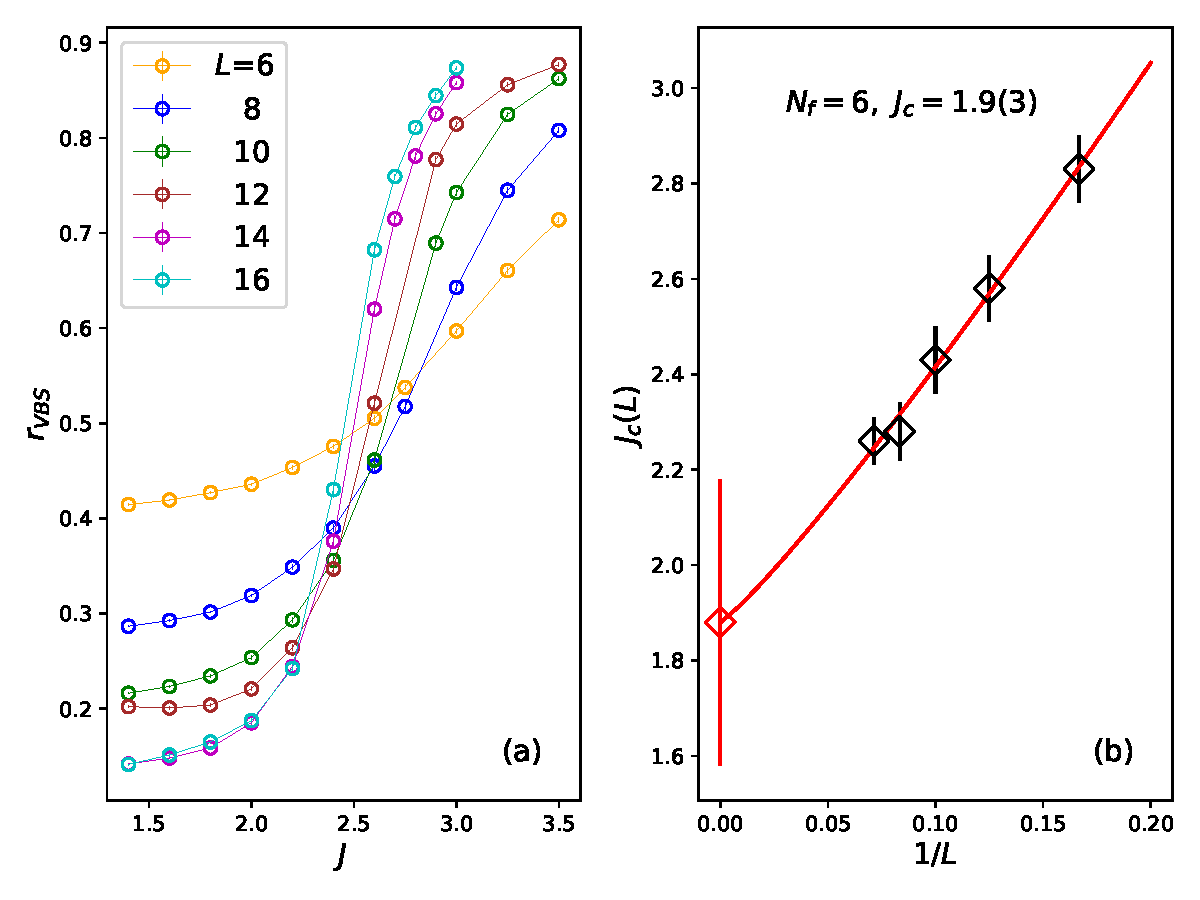
\includegraphics[width=\textwidth]{n6rvbs}
		\column{.3\textwidth}
		\begin{itemize}
			\item Phase transition b/w U1D and VBS: $J_c=1.9(3)$.
		\end{itemize}
  \end{columns}
\end{frame}

\begin{frame}
  \frametitle{$N_f=6$: U1D phase}
  \begin{columns}
		\column{.5\textwidth}
    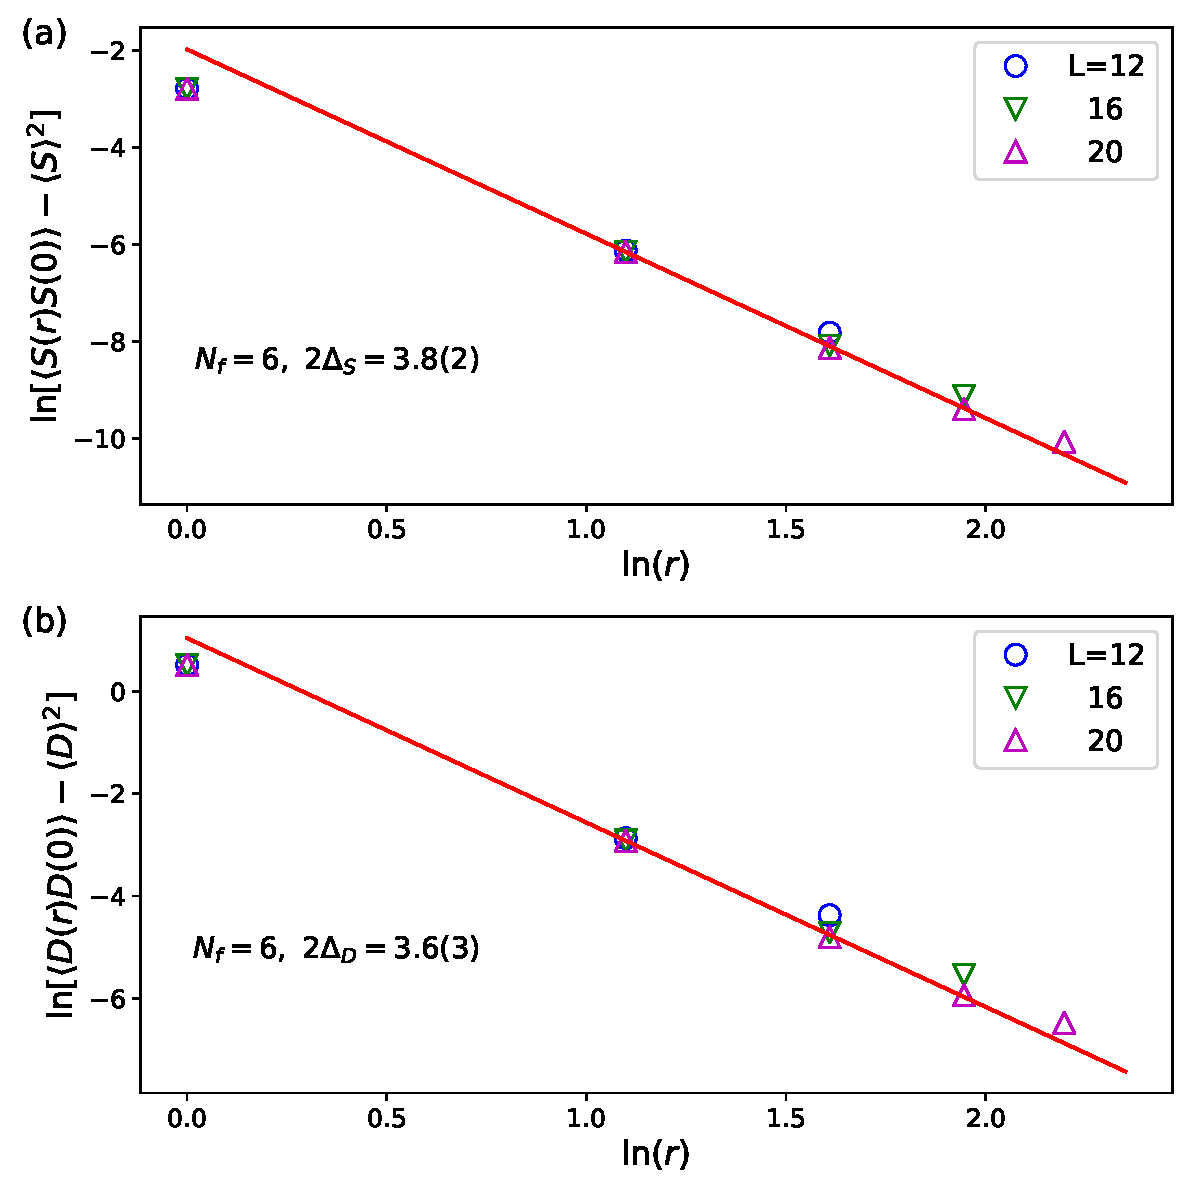
\includegraphics[width=\textwidth]{n6decay}
		\column{.5\textwidth}
		\begin{itemize}
			\item Spin and dimer OPs are fermion bilinears:
			\[\vec S = \psi^\dagger_{i\alpha}\vec\sigma_{\alpha\beta}\psi_{i\beta},\]
			\[D_{x,y} = \psi^\dagger_{i\alpha}\psi_{i+x,y,\beta}.\]
			\item Algebraic spin liquid: $\Delta_S = \Delta_D$.
		  \item (Free fermion has $\Delta_S=\Delta_D = 4$.)
		\end{itemize}
  \end{columns}
\end{frame}

\begin{frame}
  \frametitle{$N_f=8$: phase boundary}
  \begin{columns}
		\column{.7\textwidth}
    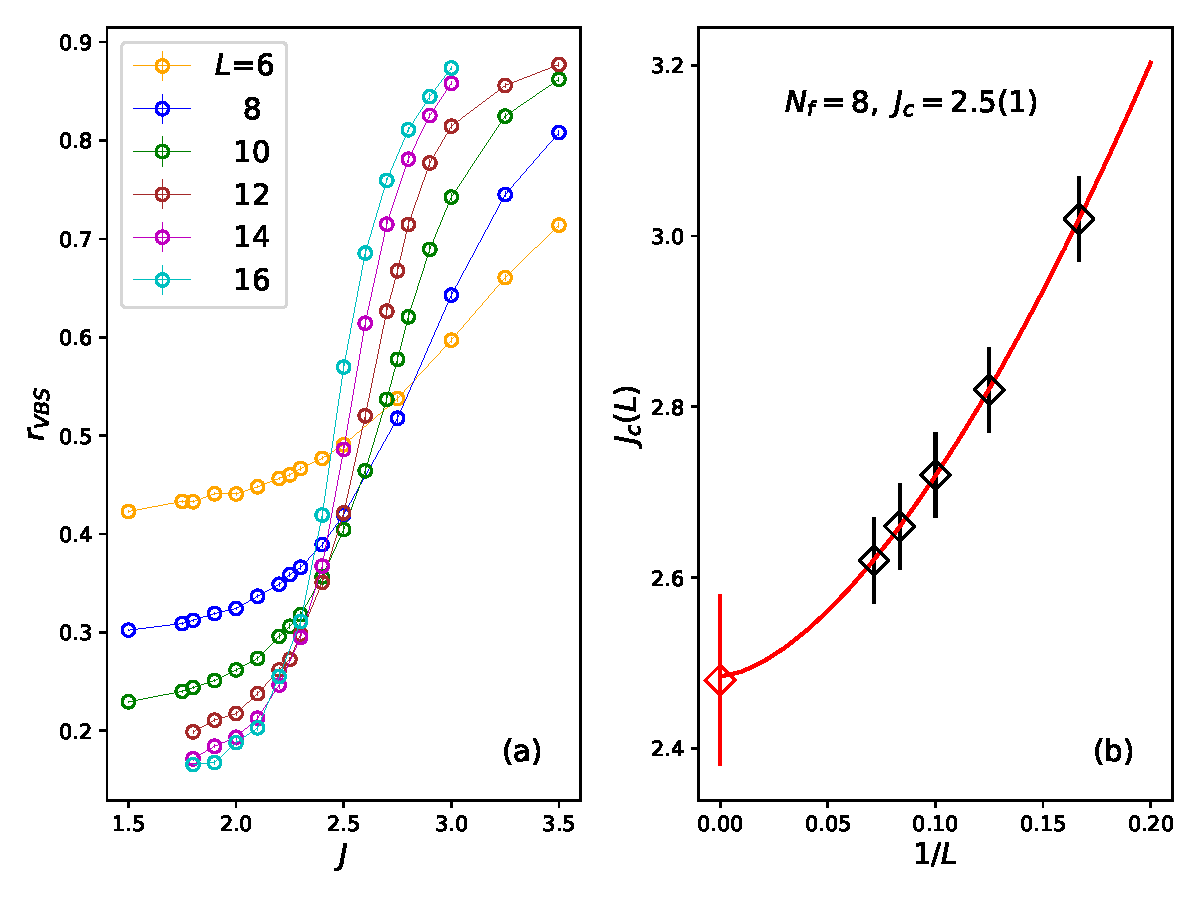
\includegraphics[width=\textwidth]{n8rvbs}
		\column{.3\textwidth}
		\begin{itemize}
			\item Phase transition b/w U1D and VBS: $J_c=2.5(1)$.
		\end{itemize}
  \end{columns}
\end{frame}

\begin{frame}
  \frametitle{$N_f=8$: U1D phase}
  \begin{columns}
		\column{.5\textwidth}
    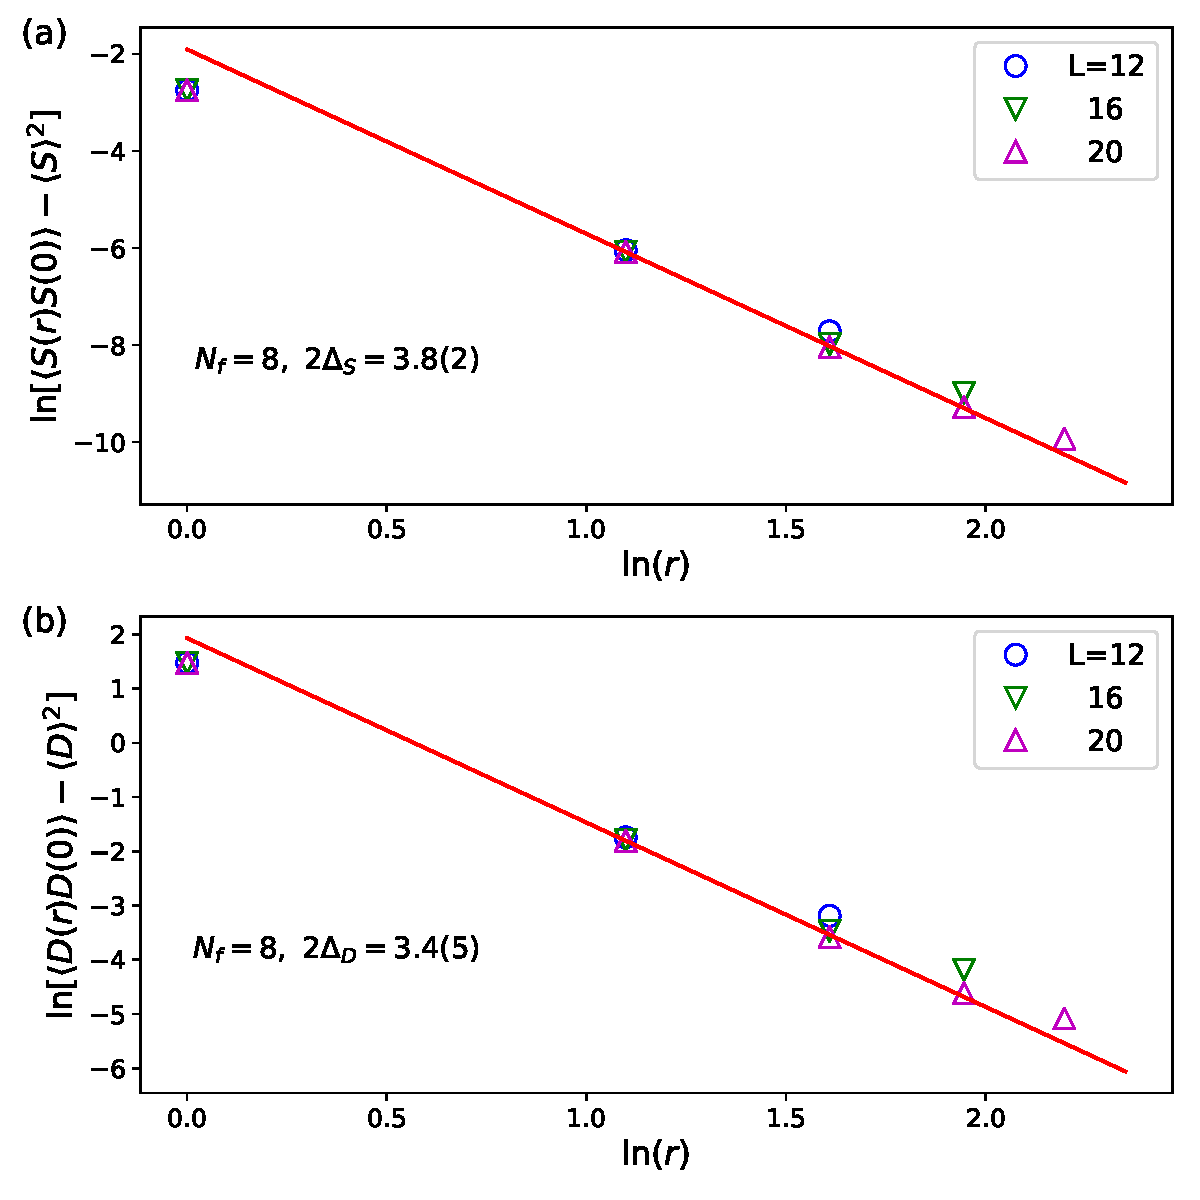
\includegraphics[width=\textwidth]{n8decay}
		\column{.5\textwidth}
		\begin{itemize}
			\item Spin and dimer OPs are fermion bilinears:
			\[\vec S = \psi^\dagger_{i\alpha}\vec\sigma_{\alpha\beta}\psi_{i\beta},\]
			\[D_{x,y} = \psi^\dagger_{i\alpha}\psi_{i+x,y,\beta}.\]
			\item Algebraic spin liquid: $\Delta_S = \Delta_D$.
		  \item (Free fermion has $\Delta_S=\Delta_D = 4$.)
		\end{itemize}
  \end{columns}
\end{frame}

\begin{frame}
  \frametitle{Summary}
  \begin{columns}
		\column{.7\textwidth}
    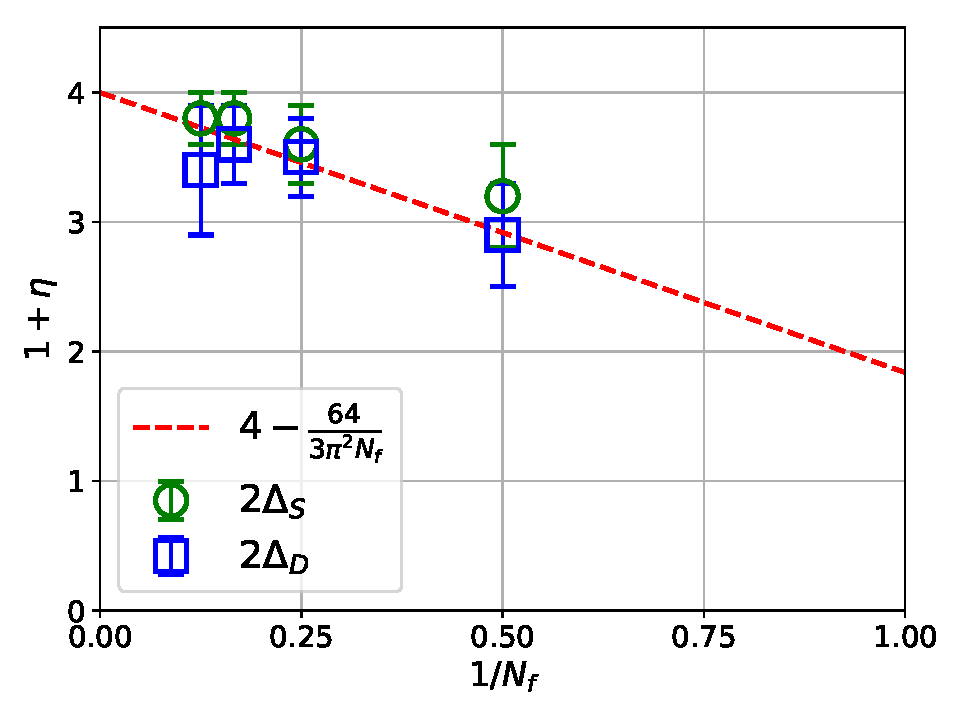
\includegraphics[width=\textwidth]{eta}
		\column{.3\textwidth}
		$\Delta_S=\Delta_D$ consistent with large-$N_f$-expansion results.
  \end{columns}
\end{frame}

\section{Conclusion}

\begin{frame}{Conclusion and outlooks}
  \begin{center}
    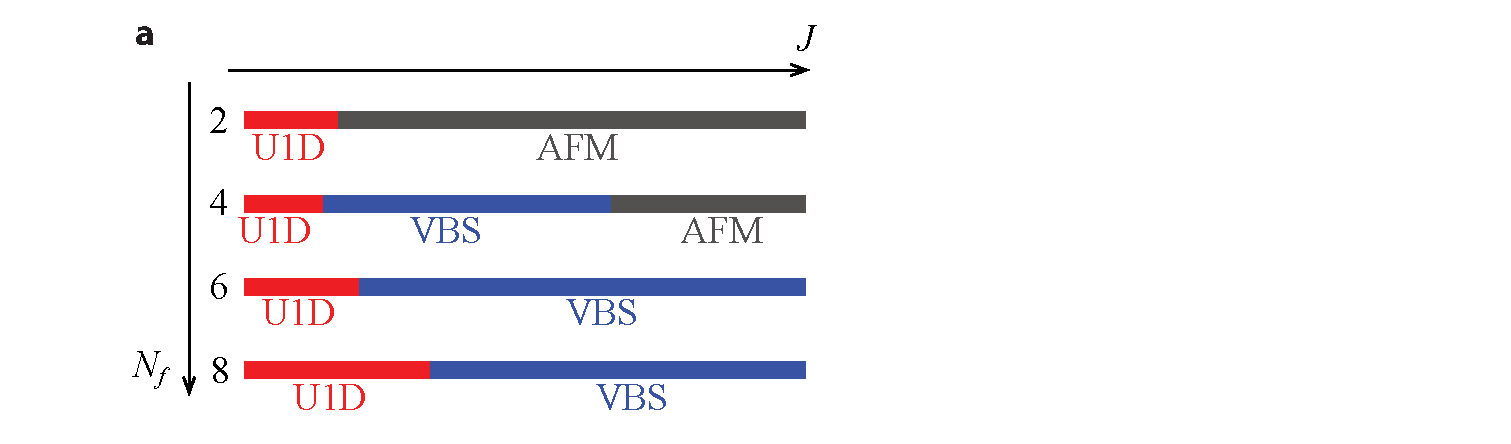
\includegraphics[width=5cm]{phase-diagram}

		{\small arXiv:1807.07574}
  \end{center}
  \begin{itemize}
    \item Deconfined U1D ASL phase observed for $N_f=2,4,6,8$.
    \item Confinement/deconfinement transition: continuous transition? universality class?
    \item Phase transition between VBS and AFM for $N_f=4$.
    \item Will U1D phase be stable in the IR limit? Larger sizes / directly measure monopole-operator scaling dimensions.
    \item Improving the algorithm: combining HMC / DQMC?
  \end{itemize}
\end{frame}

\end{document}
